\documentclass[a4paper, 12pt, oneside]{scrbook}

\usepackage[ngerman]{babel}		
\usepackage[onehalfspacing]{setspace}  %Zeilenabstand 1.5
\PassOptionsToPackage{hyphens}{url}\usepackage[hidelinks]{hyperref}

\usepackage[backend=biber,style=numeric,sorting=none]{biblatex}
\usepackage[T1]{fontenc}	  	
\usepackage[utf8]{inputenc}
\usepackage{acronym}
\usepackage[left=2.5cm,right=2.5cm,top=2.5cm,bottom=2.5cm,includeheadfoot]{geometry} % 2.5cm Randabstand werden als Minimum von der DHBW vorgeschrieben
\usepackage{graphicx}
\usepackage{epstopdf}
\usepackage{float}
\usepackage{booktabs}
\usepackage{caption}
\usepackage{csquotes}
\usepackage{fancyhdr}
\usepackage{wrapfig}
\usepackage{scrhack}

\usepackage{blindtext}
\usepackage[parfill]{parskip} % Entfernt Einrückung zu Beginn eines Paragraphen
\setkomafont{sectioning}{\normalfont\bfseries} %Schriftart für Überschriften
\setkomafont{descriptionlabel}{\normalfont\bfseries} %Schriftart für Aufzählung
\setkomafont{pageheadfoot}{\normalfont}  %Schriftart Kopfzeile nicht kursiv


\renewcommand*{\headfont}{\normalfont}
\renewcommand*{\multicitedelim}{\addsemicolon\space}
\renewcommand*{\headrulewidth}{0pt}
\renewcommand*{\arraystretch}{1.5}

\setlength{\parskip}{1.5ex}

\usepackage{comment}

% Formatierung
\usepackage{listings}
\usepackage{color}
\usepackage{hyperref}% Hyperlinks im Dokument
\hypersetup{linktoc=all} %inhaltsverzeichnis hyperlinks

\renewcommand{\lstlistingname}{Codebeispiel}
\renewcommand{\lstlistlistingname}{Codebeispielverzeichnis}

\definecolor{dkgreen}{rgb}{0,0.6,0}
\definecolor{gray}{rgb}{0.5,0.5,0.5}
\definecolor{mauve}{rgb}{0.58,0,0.82}

\lstset{frame=tb,
	language=Java,
	morekeywords={typeof, new, true, false, catch, function, return, null, catch, switch, var, if, in, while, do, else, case, break},
	ndkeywords={class, export, boolean, throw, implements, import, this, await, async},
	aboveskip=3mm,
	belowskip=3mm,
	showstringspaces=false,
	columns=flexible,
	basicstyle={\small\ttfamily},
	numbers=none,
	numberstyle=\tiny\color{gray},
	keywordstyle=\color{blue},
	commentstyle=\color{dkgreen},
	stringstyle=\color{mauve},
	breaklines=true,
	tabsize=3,
	captionpos=b
}

\bibliography{bibliography.bib}
\begin{document}

\frontmatter

% Hierin müssen Matrikelnummer Name usw. gesetzt werden.
\def\doctype{Dokumententyp}
\def\title{Entwicklung einer webbasierten Anwendung unter Verwendung des Spring Frameworks mit Test-Driven Development (TDD)}
\def\author{Isabel Lind}

\begin{titlepage}

	\vspace{10mm}

	\begin{center}
		\vspace{5mm}

		\huge \title

		\vspace{14.2pt}

		%\large \doctype


		\vspace{42.6pt}

		\large Studienarbeit T3\_3101

		\vspace{42.6pt}

		\small des Studienganges Angewandte Informatik an der \\
		\large Dualen Hochschule Baden-Württemberg Mosbach

		\vspace{14.2pt}

		
\includegraphics[height=1.5cm]{prefix/image/logo-dhbw.pdf}

		\vspace{42.6pt}

		\small von \\
		\large \author
	\end{center}

	\vspace{120pt} % 140 TODO:

	\begin{table}[h]
		\centering
		\begin{tabular}{ll}
			% \small Bearbeitungszeitraum            & XXX Wochen     \\
			\small Matrikelnummer, Kurs            & 8471449, INF21B \\
			\small Gutachter der Dualen Hochschule & Philipp Abele   \\
		\end{tabular}
	\end{table}

	\vspace{49.7pt}

	\fancypagestyle{empty}{
		\fancyhf{}
		\fancyfoot[C]{\today}
	}

\end{titlepage}

\pagenumbering{gobble}
\vspace*{100pt}

\begin{center}
	Eigenständigkeitserklärung
\end{center}

\textit{
	\noindent Ich versichere hiermit, dass ich meine Studienarbeit mit dem Thema: \\
	\glqq\title\grqq{} \\
	selbstständig verfasst und keine anderen als die angegebenen Quellen und Hilfsmittel benutzt habe. \\
	Ich versichere zudem, dass die eingereichte elektronische Fassung mit der gedruckten Fassung übereinstimmt.}

\vspace*{4em}

\hrulefill \\
Ort, Datum \hspace{8em} Unterschrift

\newpage

\tableofcontents

% Abbildungsverzeichnis
\cleardoublepage
\phantomsection
\addcontentsline{toc}{chapter}{\listfigurename}
\pagenumbering{Roman}
\listoffigures

% Tabellenverzeichnis
% \cleardoublepage
% \phantomsection
% \addcontentsline{toc}{chapter}{\listtablename}
% \listoftables

%Codebeispiel Verzeichnis
% \cleardoublepage
% \phantomsection
% \addcontentsline{toc}{chapter}{\lstlistlistingname}
% \lstlistoflistings

% Abkürzungsverzeichnis (siehe Ordner "prefix")
\chapter{Abkürzungsverzeichnis}
\begin{acronym}
	% \acro{SFC}{Single-File Component}
	% \acroplural{SFC}[SFCs]{Single-File Components}
\end{acronym}

\mainmatter

% Inhalt (siehe Ordner "content") %
\chapter{Einleitung}
\chapter{Grundlagen}
\section{Test-Driven Development}
Bei dem Test-Driven Development (TDD), zu Deutsch auch „test-getriebene Entwicklung“, handelt es sich um ein Entwicklungs- und Designverfahren für Software, bei dem Testfälle bereits vor oder spätestens parallel zur Implementierung spezifiziert werden. Die zu erstellende Software wird quasi über Tests entworfen. \cite[S. 151]{schatten_best_2010}

TDD sollte bereits bei der Anforderungsanalyse angewendet werden. Die Anforderungen sind so zu definieren, dass sichergestellt werden kann, dass die Erfüllung dieser Anforderungen mithilfe von Tests validiert werden können. Dies kann durch Testdefinitionen in Textform gewährleistet werden, in die genau die Vorbedingungen, die Ausführung und die zu erwartenden Ergebnisse beschrieben werden. \cite[S.188] {kleuker_qualitatssicherung_2019}

Die Abbildung \ref{schematischer Ablauf TDD} zeigt exemplarisch einen schematischen Ablauf des Test-Driven Development-Ansatzes. Am Anfang wird der Testfall definiert (Test Definition, TD), darauf folgt die Umsetzung und Programmierung (Programming, P). Im Anschluss werden die Testfälle ausgeführt (Test Execution, TE). \cite[S. 151]{schatten_best_2010}

\begin{figure}[h]
	\centering
	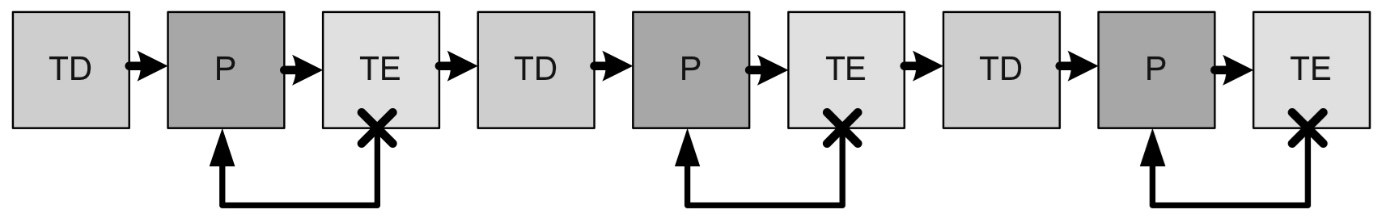
\includegraphics[clip,width=1\linewidth]{images/schematischer Ablauf TDD.jpg}
	\caption[schematischer Ablauf des Test-Driven Development]{schematischer Ablauf des Test-Driven Development \cite[S. 151]{schatten_best_2010}}
	\label{schematischer Ablauf TDD}
\end{figure}

Im Gegensatz dazu wird beim traditionellen Testen erst parallel zur Entwicklung oder nach Abschluss der Implementierung geeignete Testfälle definiert und ausgeführt, wie ein schematischer Ablauf in Abbildung \ref{schematischer Ablauf traditionelles Testen} zeigt. \cite[S. 150]{schatten_best_2010}

\begin{figure}[h]
	\centering
	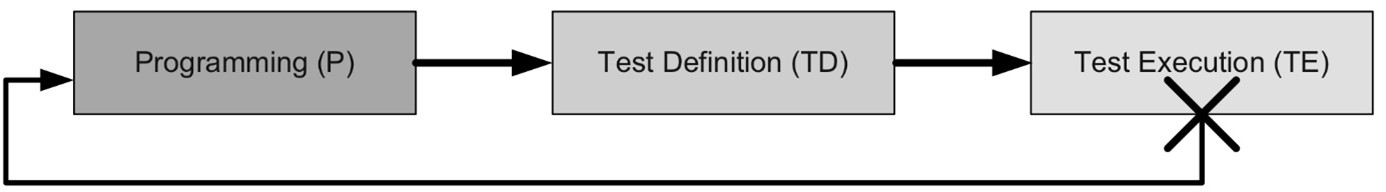
\includegraphics[clip,width=1\linewidth]{images/schematischer Ablauf traditionelles Testen.jpg}
	\caption[schematischer Ablauf des traditionellen Testen]{schematischer Ablauf des traditionellen Testen \cite[S.151]{schatten_best_2010}}
	\label{schematischer Ablauf traditionelles Testen}
\end{figure}

Durch das frühe Definieren und Ausführen von Testfällen im TDD-Ansatz erhalten die Entwickler ein unmittelbares Feedback zur erstellten Lösung und Probleme wie Seiteneffekte können frühzeitig erkannt werden \cite[S. 151]{schatten_best_2010}. 
Da der Entwickler sich für die Testerstellung intensiv mit den Anforderungen auseinander setzen muss, erhält er ein verbessertes Verständnis für das zu entwickelnden Produkt und die eigentliche Entwicklungszeit kann deutlich verkürzt werden. Die Anzahl verschleppter und dann aufwändig zu reparierender Fehler kann zudem, durch die von der Entwicklung unabhängigen Erstellung der Testfälle, reduziert werden. Denn, wenn erst nach der Implementierung die Testfälle definiert werden, besteht eine große Wahrscheinlichkeit, dass Denkfehler bei der Implementierung bei der Testerstellung wiederholt werden und somit falsche Tests, die falsche zu testende Software, als korrekt überprüfen \cite[S.188] {kleuker_qualitatssicherung_2019}.  

Die frühzeitig erstellten Tests eignen sich ferner auch zur Automatisierung und des Weiteren kann durch die Testfälle und deren Testergebnisse die Kommunikation verbessert werden. TDD wird meistens im Rahmen der agilen Software-Entwicklung verwendet und ist fester Bestandteil verschiedener Vorgehensmodelle, wie eXtreme Programming und SCRUM \cite[S. 151]{schatten_best_2010}. 

\subsection{Ablauf von Test-Driven Development}

Der entscheidende Bestandteil des Test-Driven Development ist, dass die Testfälle vor oder spätestens parallel zur Implementierung definiert werden. Im Anschluss werden die Softwarekomponenten implementiert bzw. angepasst, bis die definierten Tests erfolgreich durchlaufen. Konkret lässt sich TDD in vier grundlegende Schritte unterteilen, wie sie in Abbildung \ref{Phasen des TDD} skizziert werden. \cite[S. 153]{schatten_best_2010}

In dem ersten Schritt „think“ wird die Anforderung ausgewählt, die im nächsten Schritt umgesetzt werden soll. Anhand der ausgewählten Anforderung werden die geeigneten Tests definiert. Hierbei ist sicherzustellen, dass die ausgewählte Anforderung auch tatsächlich durch die Tests abgedeckt wird. Unit-Tests können beispielsweise auf der Implementierungsebene z.B. für Komponenten verwendet werden. \cite[S. 153]{schatten_best_2010}

In dem zweiten Schritt „red“ werden diese Tests ausgeführt. Da es noch keine Implementierung dazu gibt, schlagen die Tests fehl und sind im Status „red“. \cite[S. 153]{schatten_best_2010}

Dann erfolgt die Implementierung, bis die erstellten Tests erfolgreich durchlaufen und den Status „green“ erreichen (Schritt drei). Dabei wird die Anforderung schrittweise implementiert und getestet. Wenn die Testfälle nicht erfolgreich durchlaufen, werden Fehler korrigiert, falls die Anforderung bereits umgesetzt wurde oder die Funktionalität implementiert, falls die Anforderung noch nicht umgesetzt wurde. \cite[S. 153]{schatten_best_2010}

Im letzten Schritt erfolgt die Optimierung und Anpassung des geschriebenen Softwarecodes (vierter Schritt Refactoring). Da durch das Refactoring der Code verändert wird, müssen alle Testfälle im Anschluss jeweils durchgeführt werden, um sicherzustellen, dass alle Tests weiterhin erfolgreich durchlaufen und der Status „green“ nicht mehr verlassen wird. \cite[S. 153]{schatten_best_2010}

Wenn das Refactoring erfolgreich durchgeführt wurde, ist die Implementierung für die ausgewählte Anforderung abgeschlossen und die nächste Anforderung kann durch die gleiche Schrittfolge umgesetzt werden. \cite[S. 153 f.]{schatten_best_2010} 

\begin{figure}[h]
	\centering
	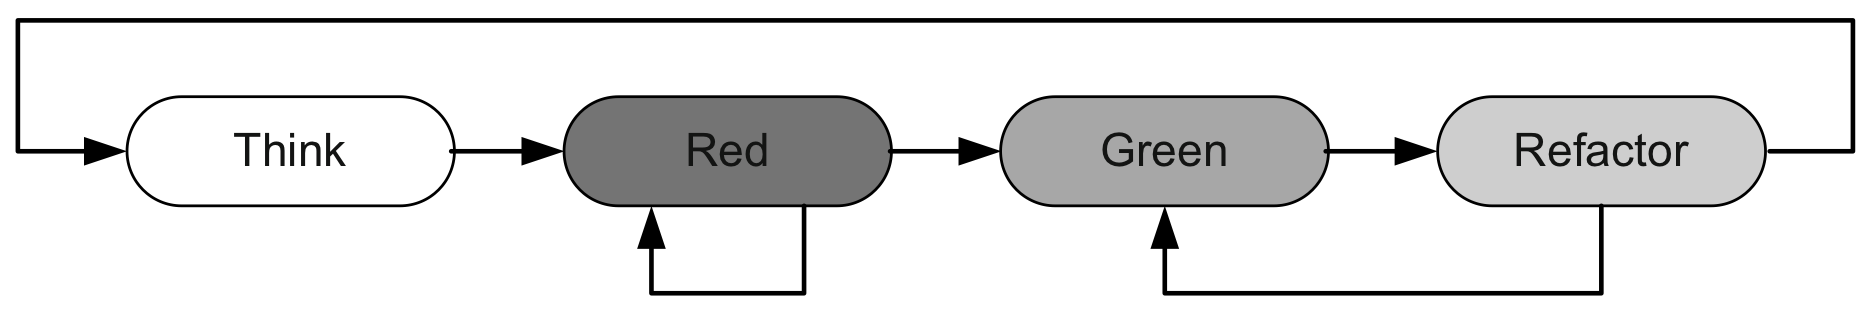
\includegraphics[clip,width=1\linewidth]{images/Phasen des TDD.png}
	\caption[Phasen des Test-Driven Development]{Phasen Ablauf des Test-Driven Development \cite[S. 153]{schatten_best_2010}}
	\label{Phasen des TDD}
\end{figure}

Die Abbildung \ref{Anwendungsbeispiel TDD} zeigt einen beispielhaften schematischen Ablaufes von TDD in der Praxis. Dabei wird veranschaulicht, dass für die ausgewählten Anforderungen geeignete Testfälle erstellt werden, um die Erfüllung der Anforderung validieren zu können. In dem Anwendungsbeispiel wird für die Anforderung A drei Testfälle benötigt. Die Testläufe, welche auf der x-Achse dargestellt werden, geben den Status der Testfälle an und wechseln von „red“ in „green“, entsprechend den jeweiligen TDD-Schritten. Dabei wird ersichtlich, dass die Anforderungen schrittweise implementiert und getestet werden. Dieses Beispiel zeigt ebenfalls auf, wie durch die schnelle Rückmeldung, durch die Tests, Seiteneffekte frühzeitig entdeckt werden können. Eine Implementierung, welche für den Testfall C2 bestimmt war, bewirkte, dass nicht nur der Test C2 weiterhin fehlschlägt, sondern auch der Testfall B2. Dieser Testfall wäre wohlmöglich bei einem traditionellen Testanfall erst sehr spät entdeckt worden und müsste aufwendig korrigiert werden. \cite[S. 154]{schatten_best_2010}

\begin{figure}[h]
	\centering
	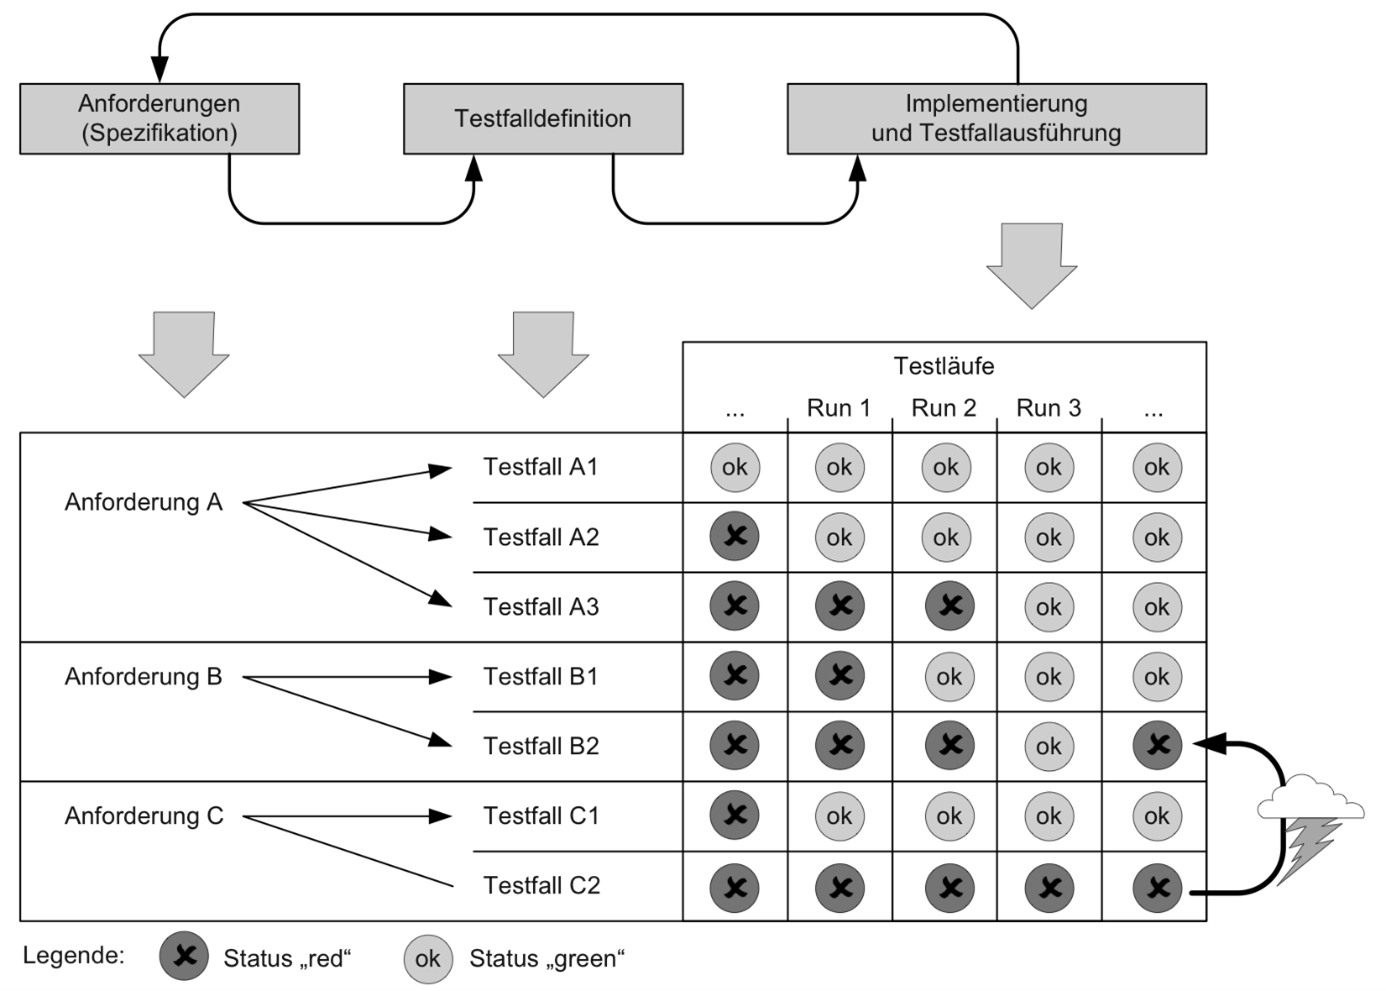
\includegraphics[clip,width=1\linewidth]{images/Anwendungsbeispiel TDD.png}
	\caption[schematischer Ablauf von Test-Driven Development in der Praxis ]{schematischer Ablauf von Test-Driven Development in der Praxis \cite[S. 154]{schatten_best_2010}}
	\label{Anwendungsbeispiel TDD}
\end{figure}

\subsection{Arten des Test-Driven Development}


\chapter{Konzeption und Design der Todo-App}
\section{Architektur der Anwendung}
Die Todo-App ist als eine mehrschichtige Architektur konzipiert, die eine klare Trennung der Verantwortlichkeiten zwischen den verschiedenen Schichten sicherstellt. Diese Architektur umfasst die folgenden Schichten:

\begin{itemize}
	\item \textbf{Präsentationsschicht}: Diese Schicht besteht aus REST-Controllern, die HTTP-Anfragen entgegennehmen und HTTP-Antworten zurückgeben. Sie interagiert mit der Service-Schicht, um Geschäftslogik zu implementieren.
	\item \textbf{Service-Schicht}: Diese Schicht enthält die Geschäftslogik der Anwendung. Sie validiert die Daten und ruft die entsprechenden Methoden der Repository-Schicht auf.
	\item \textbf{Repository-Schicht}: Diese Schicht besteht aus JPA-Repositories, die für die Datenzugriffslogik verantwortlich sind. Sie interagiert mit der MySQL-Datenbank, um Daten zu speichern und abzurufen.
	\item \textbf{Sicherheitsschicht}: Diese Schicht nutzt Spring Security, um Authentifizierung und Autorisierung zu implementieren. JWT (JSON Web Tokens) wird verwendet, um die Benutzersitzungen zu verwalten.
	\item \textbf{Datenbank-Schicht}: Diese Schicht besteht aus einer MySQL-Datenbank, in der alle Daten der Anwendung gespeichert werden.
\end{itemize}

\section{Datenmodell und Datenbankdesign}

\subsection{Entwurf des Datenmodells}
Das Datenmodell der Todo-App umfasst mehrere Entitäten, um die Beziehungen zwischen Benutzern und ihren Aufgaben zu verwalten. Die Hauptentitäten sind User und Todo.

\textbf{User Entität}

Die User-Entität repräsentiert einen Benutzer der Anwendung und enthält folgende Attribute:

\begin{itemize}
	\item id: Ein eindeutiger Bezeichner für jeden Benutzer.
	\item username: Der Benutzername, den der Benutzer zur Anmeldung verwendet.
	\item password: Das verschlüsselte Passwort des Benutzers.
\end{itemize}

Die User-Entität wird als Java-Klasse implementiert und mit JPA-Anmerkungen versehen, um die Zuordnung zur Datenbank zu erleichtern.

\begin{lstlisting}
	@Entity
	public class User {
		
		@Id
		@GeneratedValue(strategy = GenerationType.IDENTITY)
		private Long id;
		
		@Column(unique = true, nullable = false)
		private String username;
		
		@Column(nullable = false)
		private String password;
		
		// Getter und Setter
	}
\end{lstlisting}
	
\textbf{Todo Entität}

Die Todo-Entität repräsentiert eine Aufgabe und enthält folgende Attribute:

\begin{itemize}
	\item id: Ein eindeutiger Bezeichner für jede Todo.
	\item title:  Der Titel der Todo.
	\item description: Eine Beschreibung der Todo.
	\item dueDate: Das Fälligkeitsdatum der Todo.
	\item completed: Ein boolescher Wert, der angibt, ob die Todo abgeschlossen ist.
	\item user: Eine Beziehung zum Benutzer, der die Todo erstellt hat.
\end{itemize}

Die Todo-Entität wird als Java-Klasse implementiert und mit JPA-Anmerkungen versehen, um die Zuordnung zur Datenbank zu erleichtern.

\begin{lstlisting}
	@Entity
	public class Todo {
		
		@Id
		@GeneratedValue(strategy = GenerationType.IDENTITY)
		private Long id;
		
		@Column(nullable = false)
		private String title;
		
		@Column
		private String description;
		
		@Column
		private LocalDate dueDate;
		
		@Column(nullable = false)
		private boolean completed;
		
		@ManyToOne
		@JoinColumn(name = "user_id", nullable = false)
		private User user;
		
		// Getter und Setter
	}
\end{lstlisting}


%\subsection{Datenbankauswahl}

%Für die Persistenz der Daten wurde MySQL als relationales Datenbankmanagementsystem (RDBMS) ausgewählt. Die Entscheidung für MySQL basiert auf den folgenden Überlegungen:

%\begin{itemize}
	%\item \textbf{Technische Basis}: MySQL ist ein RDBMS, das Datensätze in mehreren separaten Tabellen speichert. Dies ermöglicht eine strukturierte und kodifizierte Datenspeicherung.
	%\item \textbf{Verbreitung und Unterstützung}: MySQL bietet eine hohe Kompatibilität mit verschiedenen Systemen, Programmiersprachen und Technologien, was die Integration und Verwaltung erleichtert.
	%\item \textbf{Open-Source und Flexibilität}: MySQL ist als Open-Source-Software verfügbar, was bedeutet, dass die Basissoftware frei installiert und genutzt werden kann. Der Quellcode kann von Dritten modifiziert und angepasst werden. Es gibt zudem kostenpflichtige Versionen mit erweiterten Funktionen und Dienstleistungen.
	%\item \textbf{Performance und Zuverlässigkeit}: MySQL ist für seine hohe Geschwindigkeit und Zuverlässigkeit bekannt, unterstützt durch eine große Gemeinschaft von Entwicklern. Es wurde entwickelt, um große Datenbanken effizient zu verarbeiten und wird seit vielen Jahren in produktionsreifen Anwendungen eingesetzt.
	%\item \textbf{Benutzerfreundlichkeit}: MySQL ist einfach zu installieren und zu nutzen. Viele Aufgaben können über die Befehlszeile erledigt werden, und es gibt zahlreiche Verwaltungstools wie phpMyAdmin, die eine grafische Benutzeroberfläche bieten.
	%\item \textbf{Verfügbarkeit und Sicherheit}: MySQL bietet hohe Verfügbarkeit durch Cluster-Server und Replikationskonfigurationen, die eine kontinuierliche Betriebszeit sicherstellen. Die Sicherheitsfunktionen umfassen SSL-Verschlüsselung, Datenmaskierung und Authentifizierungs-Plugins.
	%\item \textbf{Skalierbarkeit}: MySQL kann skaliert werden, um größere Datenmengen zu verarbeiten, allerdings erfordert dies technische Anpassungen. Die native Replikationsarchitektur ermöglicht es, Anwendungen zu skalieren, um eine große Anzahl von Benutzern zu unterstützen.
	%\item \textbf{Funktionsweise}: MySQL besteht aus einem Server und mehreren Clients. Der Server verwaltet die Datenbanken, während die Clients Anfragen stellen und Daten abrufen können. MySQL unterstützt verschiedene Datentypen und ermöglicht die Verwaltung von Daten über SQL.
%\end{itemize}

%Die Entscheidung für MySQL beruht auf diesen technischen und funktionalen Eigenschaften, die es zu einer geeigneten Wahl für die Anforderungen des Projekts machen.

\subsection{Projektanforderungen an die Datenbank}

Das Projekt stellt spezifische Anforderungen an die Datenbank, die durch MySQL erfüllt werden:

\begin{itemize}
	\item \textbf{Datenintegrität und Konsistenz}: Die Datenbank muss in der Lage sein, Daten in einer strukturierten und konsistenten Weise zu speichern. MySQL gewährleistet dies durch die Verwendung relationaler Tabellen und die Unterstützung von Transaktionen.
	\item \textbf{Hohe Verfügbarkeit}: Das Projekt erfordert eine Datenbank, die rund um die Uhr verfügbar ist, um eine unterbrechungsfreie Nutzung zu gewährleisten. MySQL bietet durch seine Cluster- und Replikationsfunktionen eine hohe Verfügbarkeit.
	\item \textbf{Skalierbarkeit}: Das Projekt muss in der Lage sein, mit wachsendem Datenvolumen und steigender Benutzeranzahl zu skalieren. MySQL kann durch seine Replikationsarchitektur und die Möglichkeit zur Anpassung an größere Datenmengen skaliert werden.
	\item \textbf{Sicherheit}: Der Schutz sensibler Daten ist von entscheidender Bedeutung. MySQL bietet umfassende Sicherheitsfunktionen wie SSL-Verschlüsselung, Datenmaskierung und Authentifizierungs-Plugins, um die Datensicherheit zu gewährleisten.
	\item \textbf{Performance}: Das Projekt erfordert schnelle Datenverarbeitungszeiten, um eine reibungslose Benutzererfahrung zu gewährleisten. MySQL bietet eine hohe Geschwindigkeit und Effizienz bei der Verarbeitung großer Datenbanken.
	\item \textbf{Flexibilität und Integration}: Die Datenbank muss flexibel genug sein, um mit verschiedenen Programmiersprachen und Technologien integriert zu werden. MySQL bietet eine breite Unterstützung für verschiedene Systeme und Schnittstellen.
	\item \textbf{Benutzerfreundlichkeit}: Eine einfache Installation und Verwaltung der Datenbank ist erforderlich, um den Entwicklungsprozess zu optimieren. MySQL ist benutzerfreundlich und bietet zahlreiche Verwaltungstools, die die Bedienung erleichtern.
\end{itemize}

Diese Anforderungen des Projekts werden durch die funktionalen und technischen Merkmale von MySQL umfassend abgedeckt, was die Entscheidung für MySQL als Datenbanklösung rechtfertigt.


\subsection{Datenbankdesign}

Das Datenbankdesign umfasst zwei Tabellen: users und todos. Die Struktur der Tabellen ist wie folgt:

Tabelle users
\begin{itemize}
	\item id (BIGINT, AUTO\_INCREMENT, PRIMARY KEY)
	\item username (VARCHAR, NOT NULL, UNIQUE)
	\item password (VARCHAR, NOT NULL)
\end{itemize}

Tabelle todos
\begin{itemize}
	\item id (BIGINT, AUTO\_INCREMENT, PRIMARY KEY)
	\item title (VARCHAR, NOT NULL)
	\item description (TEXT)
	\item dueDate (DATE)
	\item completed (BOOLEAN, NOT NULL)
	\item user\_id (BIGINT, FOREIGN KEY)
\end{itemize}

Durch diese Struktur wird sichergestellt, dass jede Aufgabe eindeutig einem Benutzer zugeordnet ist. Diese Beziehung ermöglicht es, dass Benutzer nur ihre eigenen Todos sehen und verwalten können.

\section{User Interface Design}

\subsection{Gestaltung der Benutzeroberfläche}

Die Benutzeroberfläche der Todo-App ist so gestaltet, dass sie intuitiv und benutzerfreundlich ist. Die Anwendung besteht aus mehreren Ansichten, die jeweils spezifische Funktionen bereitstellen:

\begin{itemize}
	\item \textbf{/index}: Die Startseite der Anwendung siehe Abbildung \ref{UI_index}. Diese Seite bietet zwei Hauptoptionen: "`Log in"' und "`Sign up"'. Dies ermöglicht neuen Benutzern die Registrierung und bestehenden Benutzern die Anmeldung.
	
	\begin{figure}[h]
		\centering
		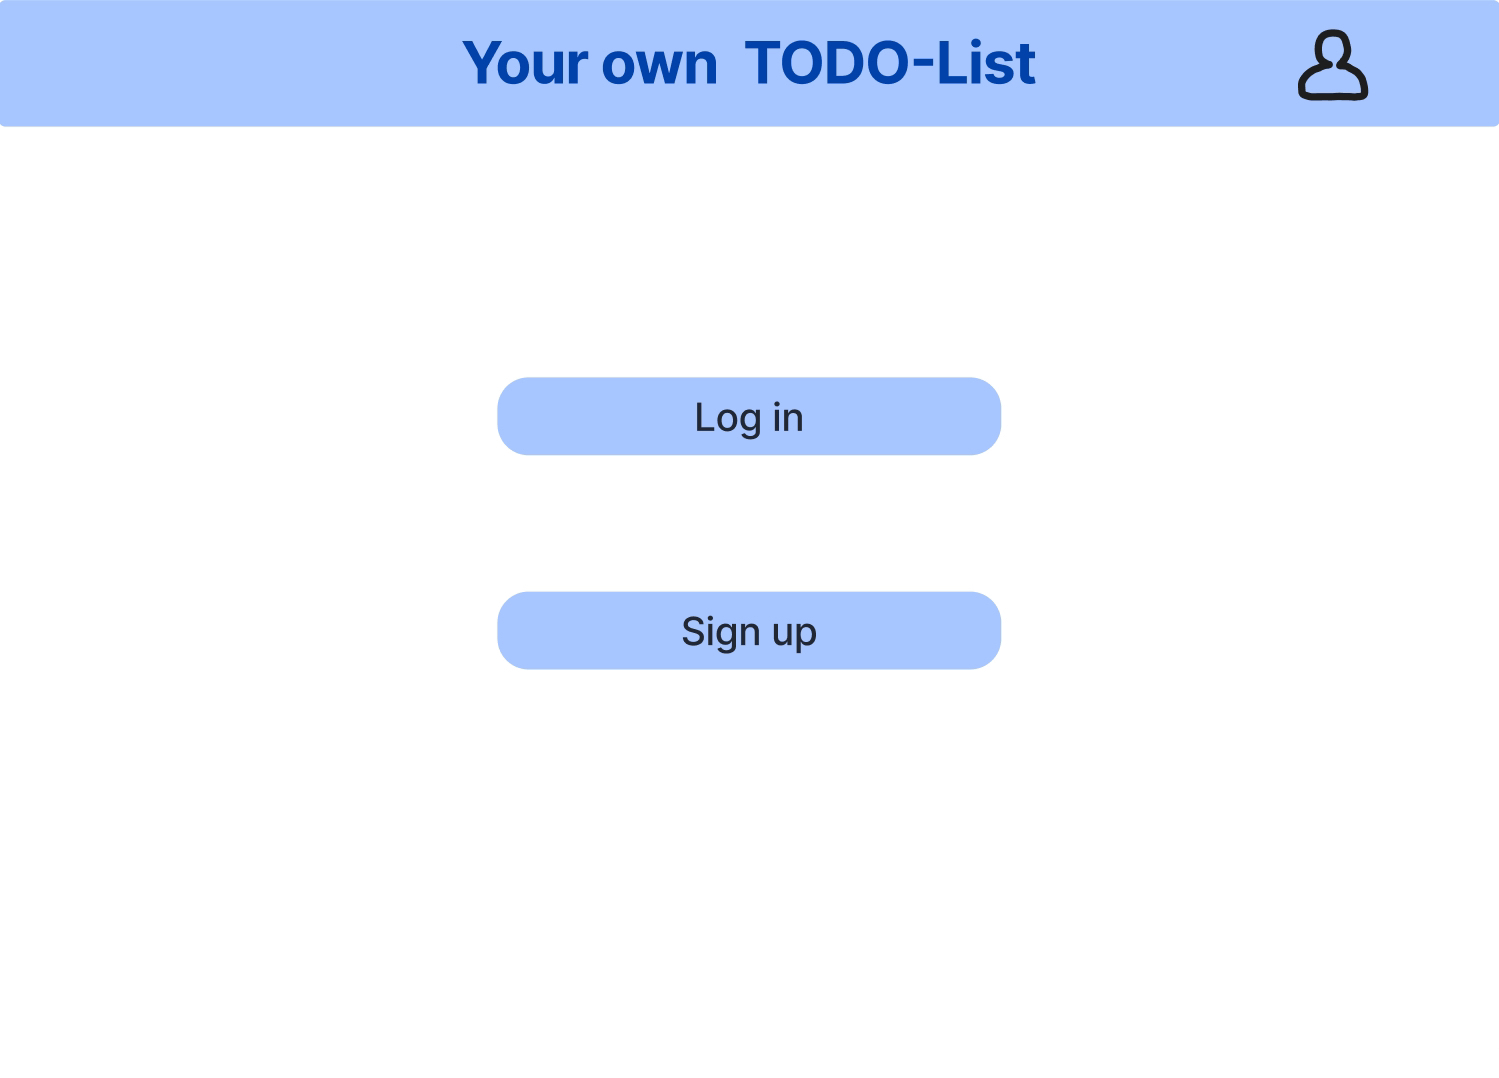
\includegraphics[clip,width=0.75\linewidth]{images/index.png}
		\caption[User Interface Design der Startseite]{User Interface Design der Startseite [Eigene Darstellung]}
		\label{UI_index}
	\end{figure}	
	
	\item \textbf{/login}: Die Anmeldeseite siehe Abbildung \ref{UI_logIn}. Hier können Benutzer ihren Benutzernamen und ihr Passwort eingeben, um auf ihre persönlichen Aufgabenlisten zuzugreifen. Ein Link zur Registrierung ist ebenfalls vorhanden.
	
	\begin{figure}[h]
		\centering
		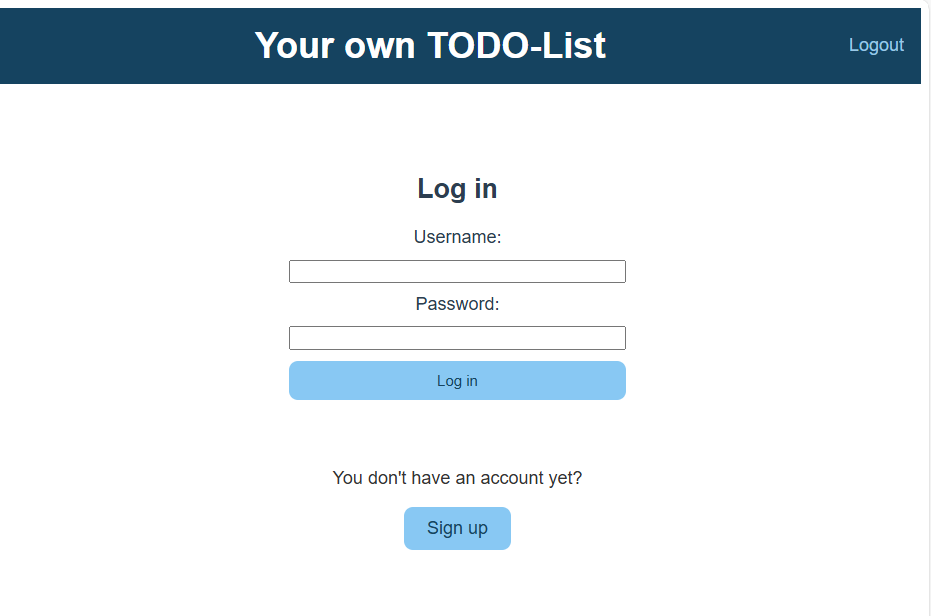
\includegraphics[clip,width=0.75\linewidth]{images/logIn.png}
		\caption[User Interface Design der Anmeldeseite]{User Interface Design der Anmeldeseite [Eigene Darstellung]}
		\label{UI_logIn}
	\end{figure}	
	
	\item \textbf{/signup}: Die Registrierungsseite siehe Abbildung \ref{UI_signUp}. Neue Benutzer können hier ein Konto erstellen, indem sie ihren Benutzernamen, ihr Passwort und die Bestätigung des Passworts eingeben. Ein Link zur Anmeldung für bestehende Benutzer ist ebenfalls verfügbar.
	
	\begin{figure}[h]
		\centering
		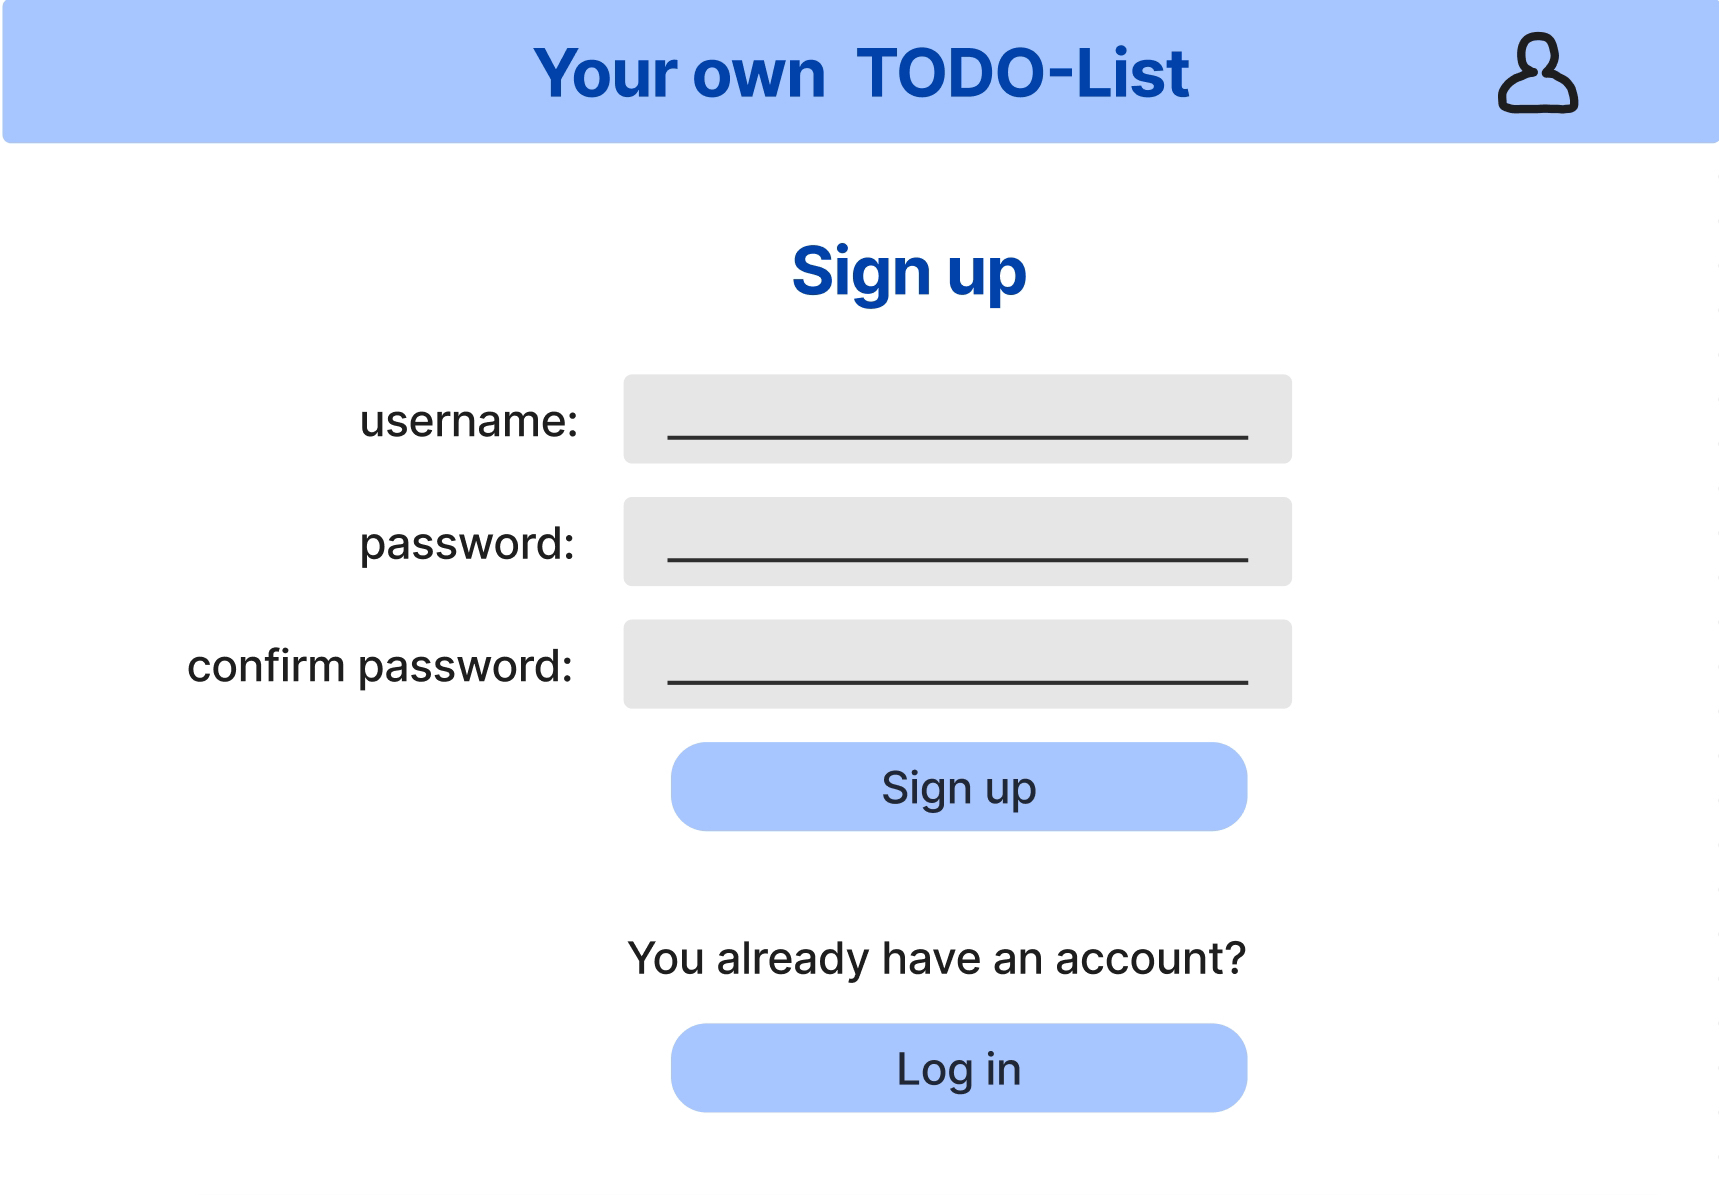
\includegraphics[clip,width=0.75\linewidth]{images/signUp.png}
		\caption[User Interface Design der Registrierungsseite]{User Interface Design der Registrierungsseite [Eigene Darstellung]}
		\label{UI_signUp}
	\end{figure}	
	
	\item \textbf{/home}: Die Hauptseite nach der Anmeldung siehe Abbildung \ref{UI_home}. Diese Seite zeigt die Aufgabenliste des angemeldeten Benutzers. Benutzer können neue Aufgaben erstellen, vorhandene Aufgaben bearbeiten oder löschen.
	
	\begin{figure}[h]
		\centering
		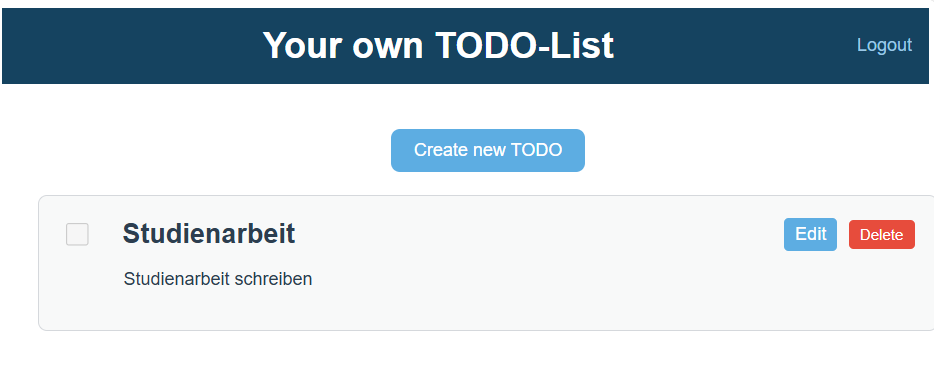
\includegraphics[clip,width=0.75\linewidth]{images/home.png}
		\caption[User Interface Design der Hauptseite]{User Interface Design der Hauptseite [Eigene Darstellung]}
		\label{UI_home}
	\end{figure}	
	
	\item \textbf{/{id\_Todo}}: Die Detailansicht einer spezifischen Todo siehe Abbildung \ref{UI_idTodo}. Diese Seite ermöglicht es Benutzern, die Details einer ausgewählten Todo zu bearbeiten.
	
	\begin{figure}[h]
		\centering
		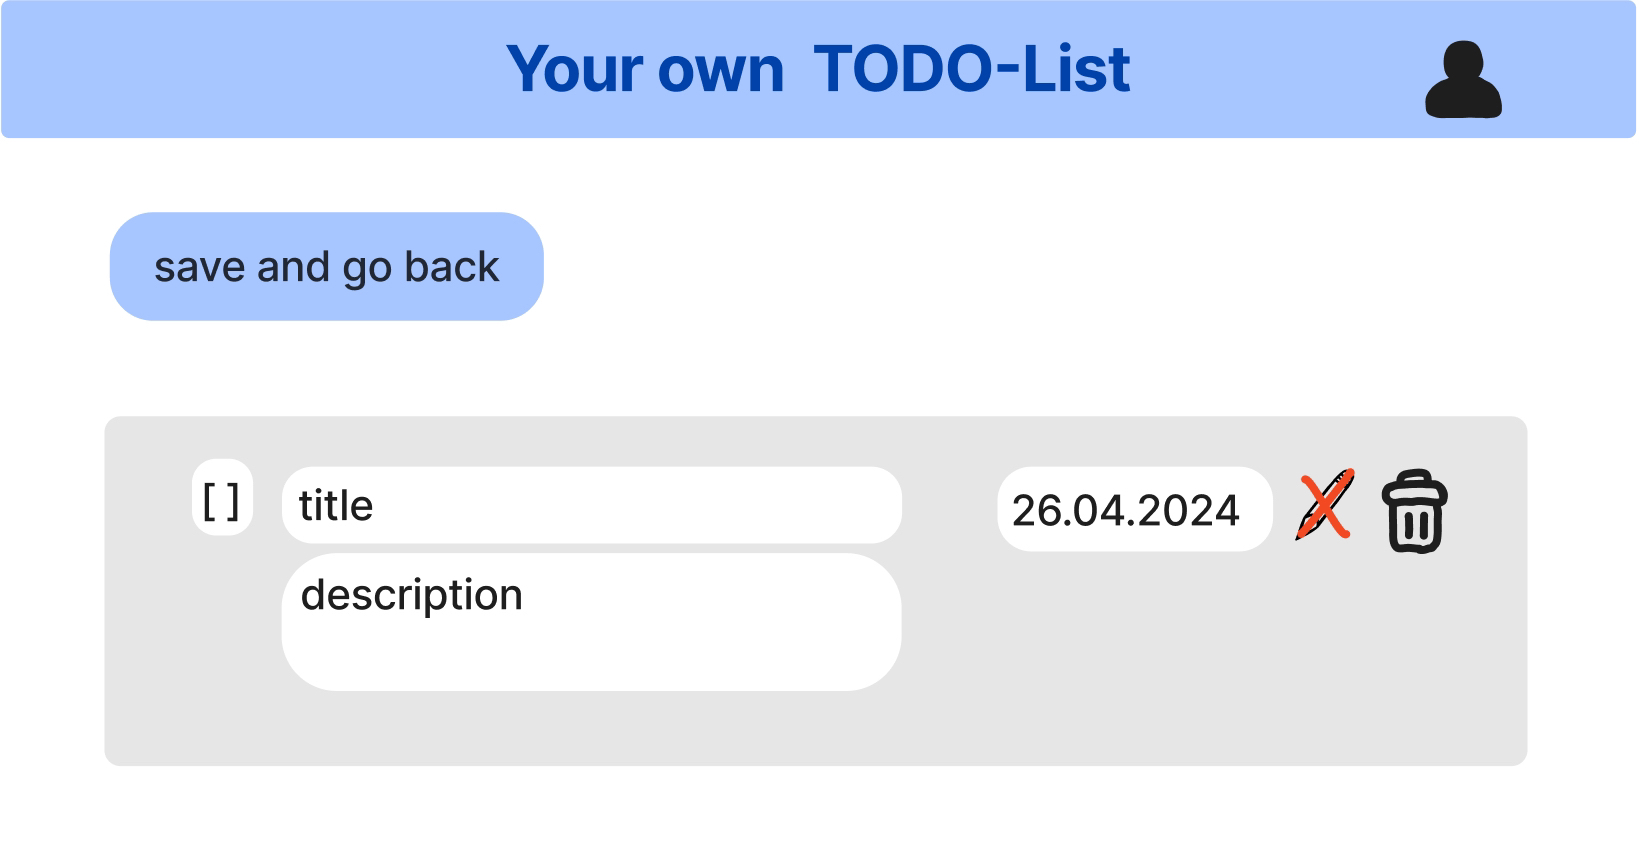
\includegraphics[clip,width=0.75\linewidth]{images/idTodo.png}
		\caption[User Interface Design der Detailansicht]{User Interface Design der Detailansicht [Eigene Darstellung]}
		\label{UI_idTodo}
	\end{figure}	
	
\end{itemize}

Jede Seite hat ein konsistentes Layout mit einem zentralen Header, der den Titel "`Your own TODO-List"' und ein Benutzer-Icon enthält. Das Benutzer-Icon signalisiert, ob ein Benutzer angemeldet ist, indem das Icon ausgefüllt ist oder, ob sich der Benutzer noch nicht angemeldet hat (unausgefülltes Icon). Bei dem drüberhoovern über das ausgefüllt Benutzer-Icon Symbol bietet sich die Möglichkeit zum abmelden ("`log out"') des angemeldeten Benutzers. 

\subsection{Berücksichtigung von Usability-Prinzipien}

Das User Interface Design der Todo-App folgt mehreren grundlegenden Usability-Prinzipien nach Jakob Nielsen, um sicherzustellen, dass die Anwendung einfach zu bedienen und effizient ist:

\begin{enumerate}
	\item \textbf{Sichtbarkeit des Systemstatus}: Die App hält den Benutzer stets über den aktuellen Status und die Ergebnisse ihrer Aktionen informiert. Beispielsweise werden Änderungen an Aufgaben sofort angezeigt und erfolgreiche Anmeldungen führen direkt zur Hauptseite mit der Aufgabenliste.
	\item \textbf{Übereinstimmung zwischen System und realer Welt}: Die Anwendung verwendet Begriffe und Konzepte, die den Benutzern vertraut sind. Schaltflächen und Symbole sind intuitiv und leicht verständlich, was die Bedienung erleichtert.
	\item \textbf{Benutzerkontrolle und Freiheit}: Benutzer können Aktionen rückgängig machen. Es gibt deutlich sichtbare Optionen zum Abbrechen von Aktionen, um Fehlaktionen leicht korrigieren zu können.
	\item \textbf{Konsistenz und Standards}: Das Layout und das Design der Benutzeroberfläche sind auf allen Seiten der Anwendung konsistent. Dies erleichtert den Benutzern das Verständnis und die Navigation durch die App.
	%\item \textbf{Fehlervermeidung}: Die Anwendung enthält Sicherheitsabfragen und Bestätigungsdialoge, um unbeabsichtigte Aktionen zu verhindern. Beispielsweise wird vor dem Löschen einer Aufgabe eine Bestätigung eingeholt.
	% TODO: mit rein nehmen, wenn es sicherheitsabfragen gibt
	\item \textbf{Wiedererkennung statt Erinnerung}: Die Benutzeroberfläche macht alle wichtigen Optionen und Funktionen sichtbar, damit Benutzer sie leicht wiedererkennen können, anstatt sich an sie erinnern zu müssen. Wichtige Elemente wie Schaltflächen und Eingabefelder sind prominent platziert und leicht zu finden. Der Einsatz von Farben und Schriftgrößen hilft, die Aufmerksamkeit der Benutzer auf wichtige Aktionen und Informationen zu lenken.
	%\item \textbf{Flexibilität und Effizienz der Nutzung}: 
	\item \textbf{Ästhetik und minimalistisches Design}: Das Design ist einfach und übersichtlich gehalten, um die Benutzerfreundlichkeit zu erhöhen. Unnötige Elemente wurden vermieden, um Ablenkungen zu minimieren und den Fokus auf die Hauptfunktionen der Anwendung zu legen.
	%\item \textbf{Hilfe beim Erkennen, Diagnostizieren und Beheben von Fehlern}: Fehlernachrichten sind in einfacher Sprache verfasst und bieten klare Hinweise zur Problemlösung. Beispielsweise wird bei einer fehlerhaften Anmeldung eine verständliche Fehlermeldung angezeigt und mögliche Lösungen vorgeschlagen.
	% TODO: Fehlermeldungen und Lösungsmöglichkeiten
	%\item \textbf{Hilfe und Dokumentation}: Obwohl die App so gestaltet ist, dass sie intuitiv bedienbar ist, steht den Benutzern bei Bedarf eine leicht durchsuchbare Hilfedokumentation zur Verfügung. Diese enthält konkrete Anleitungen zur Durchführung von Aufgaben.
\end{enumerate}

%\begin{enumerate}
%\item \textbf{Konsistenz}: Das Layout und das Design der Benutzeroberfläche sind auf allen Seiten der Anwendung konsistent. Dies erleichtert den Benutzern das Verständnis und die Navigation durch die App.
%\item \textbf{Einfache Navigation}: Die Anwendung bietet klare und sichtbare Navigationselemente. Links und Schaltflächen sind eindeutig beschriftet und führen den Benutzer durch die verschiedenen Schritte, wie Anmeldung, Registrierung und Verwaltung der Aufgaben.
%\item \textbf{Feedback}: Die App gibt dem Benutzer sofortiges Feedback auf seine Aktionen. Beispielsweise werden Änderungen an Aufgaben sofort angezeigt, und erfolgreiche Anmeldungen führen direkt zur Hauptseite mit der Aufgabenliste.
%\item \textbf{Zugänglichkeit}: Alle Eingabefelder und Schaltflächen sind groß genug und gut platziert, um sowohl auf Desktop- als auch auf mobilen Geräten leicht zugänglich zu sein.
%\item \textbf{Visuelle Hierarchie}: Wichtige Elemente wie Schaltflächen und Eingabefelder sind prominent platziert und leicht zu finden. Der Einsatz von Farben und Schriftgrößen hilft, die Aufmerksamkeit der Benutzer auf wichtige Aktionen und Informationen zu lenken.
%\item \textbf{Minimalistisches Design}: Das Design ist einfach und nicht überladen, was die Benutzerfreundlichkeit erhöht. Unnötige Elemente wurden vermieden, um die Ablenkung zu minimieren und den Fokus auf die Hauptfunktionen der Anwendung zu legen.
%\end{enumerate}




\chapter{Implementierung unter Verwendung von TDD}

\section{Entwicklungsumgebung und Werkzeuge}

Die Entwicklung der Todo-App erfolgte in einer modernen Java-Entwicklungsumgebung, die auf dem Spring Boot Framework basiert. Die wichtigsten verwendeten Tools und Technologien sind:

\begin{itemize}
	\item \textbf{IDE}: IntelliJ IDEA wurde als Integrated Development Environment (IDE) verwendet, da es umfangreiche Unterstützung für Java und das Spring Framework bietet, einschließlich leistungsstarker Debugging- und Refactoring-Tools.
	\item \textbf{Build-Tool}: Maven wurde für das Build-Management und die Abhängigkeitsverwaltung eingesetzt. Es ermöglicht die einfache Verwaltung von Bibliotheken und Plugins sowie die Konfiguration von Build-Prozessen.
	\item \textbf{Versionierung}: Git und GitHub wurden für die Quellcodeverwaltung und Versionskontrolle verwendet. GitHub ermöglichte zudem die Zusammenarbeit und den Austausch von Code.
	\item \textbf{Test-Frameworks}: JUnit 5 und Spring Boot Test wurden für die Implementierung und Ausführung von Unit- und Integrationstests verwendet. Mockito diente zur Erstellung von Mock-Objekten für die Isolierung von Testfällen.
	\item \textbf{Datenbank}: MySQL wurde als relationale Datenbank verwendet. Für die Tests wurde eine MySQL-Testdatenbank konfiguriert, um schnelle und isolierte Testausführungen zu ermöglichen.
\end{itemize}

\section{Implementierungsschritte}

Die Implementierung der Benutzerregistrierung in der Todo-App folgte dem klassischen TDD-Zyklus: \textbf{Red-Green-Refactor}.

\begin{enumerate}
	\item \textbf{Red Phase}: Zunächst wurde ein fehlgeschlagener Test (Red) geschrieben, der die Registrierung eines neuen Benutzers beschreibt, ohne dass die Implementierung vorhanden war.
	
	Beispiel: Ein Test für die Registrierung eines neuen Benutzers über den UserController.
	\begin{lstlisting}[language=Java]
		@Test
		public void testRegisterUser_success() throws Exception {
			UserRegistrationRequest request = new UserRegistrationRequest();
			request.setUsername("integrationtestuser");
			request.setPassword("password");
			request.setConfirmPassword("password");
			
			ResultActions result = mockMvc.perform(post("/register")
			.contentType(MediaType.APPLICATION_JSON)
			.content(objectMapper.writeValueAsString(request)));
			
			result.andExpect(status().isOk());
		}
	\end{lstlisting}
	
	\item \textbf{Green Phase}: Anschließend wurde der minimal notwendige Code geschrieben, um den Test erfolgreich zu bestehen (Green). In diesem Schritt wird nur so viel implementiert, dass der Testfall erfüllt wird.
	
	Beispiel: Die grundlegende Implementierung des registerUser-Endpunkts im UserController.
	
	\begin{lstlisting}[language=Java]
		@PostMapping("/register")
		public ResponseEntity<?> registerUser(@RequestBody UserRegistrationRequest request) {
			User user = new User();
			user.setUsername(request.getUsername());
			user.setPassword(passwordEncoder.encode(request.getPassword()));
			
			return ResponseEntity.ok(user);
		}
	\end{lstlisting}
	
	\item \textbf{Refactor Phase}: Nach dem erfolgreichen Bestehen des Tests wurde der Code optimiert und verbessert, ohne die Funktionalität zu ändern. Dabei wurde auf Sauberkeit, Lesbarkeit und Wartbarkeit des Codes geachtet.
	
	Beispiel: Die vollständige Implementierung des registerUser-Endpunktes im UserController zeigt, dass ein Refactoring erfolgte, nachdem die Implementierung zum erfolgreichen Ausführen von Test, wie zum Beispiel des Testens der Fehlerbehandlung von bereits existierenden Benutzernamen, hinzugefügt wurde.
	
	\begin{lstlisting}[language=Java]
		@PostMapping("/register")
		public ResponseEntity<?> registerUser(@Valid @RequestBody UserRegistrationRequest request, BindingResult result) {
			// Check if username already exists
			if (userService.existsByUsername(request.getUsername())) {
				return ResponseEntity.status(HttpStatus.CONFLICT).body("Username already exists");
			}
			
			// Check if password and confirmation match
			if (!request.getPassword().equals(request.getConfirmPassword())) {
				
				return ResponseEntity.status(HttpStatus.CONFLICT).body("Password and confirm password do not match");
			}
			
			// Check for validation results
			if (result.hasErrors()) {
				
				return ResponseEntity.status(HttpStatus.BAD_REQUEST).body("Validation error: " + result.getAllErrors());
			}
			
			// Register user
			try {
				User user = authenticationService.register(request);
				return ResponseEntity.ok(user);
			} catch (Exception e) {
				return ResponseEntity.status(HttpStatus.INTERNAL_SERVER_ERROR).body("Error registering user");
			}
		}
	\end{lstlisting}
	
\end{enumerate}

Die konsequente Anwendung des TDD-Zyklus gewährleistet, dass die Implementierung kontinuierlich durch Tests begleitet und abgesichert wird und somit zu einem stabilen und fehlerarmen Code führen kann.

\section{Beispieltests und Testfälle}

\section{Unit-Tests}

Unit-Tests wurden verwendet, um einzelne Komponenten isoliert zu testen. Ein Beispiel ist der Test der \texttt{UserController}-Klasse, um sicherzustellen, dass eine Registrierung eines Benutzers erfolgreich verläuft.

\begin{lstlisting}[language=Java]
	@Test
	public void testRegisterUserPasswordMismatch() {
		UserRegistrationRequest request = new UserRegistrationRequest("testuser", "password1", "password2");
		
		BindingResult result = mock(BindingResult.class);
		ResponseEntity<?> response = userController.registerUser(request, result);
		
		assertEquals(HttpStatus.CONFLICT, response.getStatusCode());
		assertEquals("Password and confirm password do not match", response.getBody());
	}
\end{lstlisting}

\section{Integrationstests}

Integrationstests wurden durchgeführt, um das Zusammenspiel verschiedener Komponenten zu überprüfen. Ein Beispiel ist der Integrationstest für die Benutzerregistrierung über den \texttt{UserController}.

\begin{lstlisting}[language=Java]
	@SpringBootTest(webEnvironment = SpringBootTest.WebEnvironment.RANDOM_PORT)
	public class UserRegistrationAcceptanceTest {
		
		@LocalServerPort
		private int port;
		
		@Autowired
		private TestRestTemplate restTemplate;
		
		@Test
		public void testRegisterUser() {
			String url = "http://localhost:" + port + "/register";
			UserRegistrationRequest request = new UserRegistrationRequest("testuser", "password", "password");
			
			HttpHeaders headers = new HttpHeaders();
			HttpEntity<UserRegistrationRequest> entity = new HttpEntity<>(request, headers);
			
			// Send HTTP POST request
			ResponseEntity<String> response = restTemplate.exchange(url, HttpMethod.POST, entity, String.class);
			
			// Check if the response status code is 409 (CONFLICT)
			assertEquals(HttpStatus.CONFLICT, response.getStatusCode());
		}
	}
\end{lstlisting}


\section{Akzeptanztests}

Akzeptanztests wurden verwendet, um sicherzustellen, dass die Anwendung den Anforderungen der Benutzer entspricht. Diese Tests wurden aus der Sicht des Endbenutzers geschrieben und überprüfen die Funktionalität der gesamten Anwendung.

Ein Beispiel ist der Akzeptanztest für die Benutzerregistrierung über die REST-Schnittstelle.


\begin{lstlisting}[language=Java]
	@SpringBootTest(webEnvironment = SpringBootTest.WebEnvironment.RANDOM_PORT)
	public class UserRegistrationAcceptanceTest {
		
		@LocalServerPort
		private int port;
		
		@Autowired
		private TestRestTemplate restTemplate;
		
		@Test
		public void testRegisterUser() {
			String url = "http://localhost:" + port + "/register";
			UserRegistrationRequest request = new UserRegistrationRequest("testuser", "password", "password");
			
			HttpHeaders headers = new HttpHeaders();
			HttpEntity<UserRegistrationRequest> entity = new HttpEntity<>(request, headers);
			
			// Send HTTP POST request
			ResponseEntity<String> response = restTemplate.exchange(url, HttpMethod.POST, entity, String.class);
			
			// Check if the response status code is 409 (CONFLICT)
			assertEquals(HttpStatus.CONFLICT, response.getStatusCode());
		}
	}
\end{lstlisting}

Diese strukturierte Vorgehensweise durch TDD führte zu einer robusten und fehlerarmen Implementierung der Todo-App, da jedes Feature durch entsprechende Tests abgesichert und validiert wurde.



\backmatter
\sloppy
\printbibliography
\addcontentsline{toc}{chapter}{Literaturverzeichnis}

\end{document}